%! TeX program = lualatex
\documentclass[]{beamer} 
\usetheme{SimpleDarkBlue}

% \setbeamercolor{title}{fg=black}
% \setbeamercolor{frametitle}{fg=black}
% \setbeamercolor{caption}{fg=black}
% \setbeamercolor{caption name}{fg=black}

% \setbeamertemplate{navigation symbols}{}
% \setbeamertemplate{itemize item}{\color{black}$\bullet$}

% packages
\usepackage{fontspec}
% \setmainfont{EB Garamond}
% \usefonttheme{serif}
\setmonofont[Scale=MatchLowercase]{Deja Vu Sans Mono}

\usepackage{microtype}      % Slightly tweak font spacing for aesthetics
\usepackage[english]{babel} % Language hyphenation and typographical rules

\usepackage{minted}
\usemintedstyle{algol_nu}
\usepackage{xcolor}

\usepackage{pgfplots}
\pgfplotsset{width=\textwidth,compat=1.9}

\usepackage{caption}
\newenvironment{code}{\captionsetup{type=listing, skip=0pt}}{}

\usepackage[yyyymmdd]{datetime}
\renewcommand{\dateseparator}{--}

\author{Andrew Hayes }
\title{CT437 Assignment 1}
\subtitle{Ethical Hacking \& Penetration Testing using Kali Linux \& Metasploit}
\institute{Student ID: 21321503}

\begin{document}
\frame{\titlepage}

\begin{frame}{Introduction}
    \textbf{Metasploit} is an open-source penetration testing framework that is widely used for:
    \begin{itemize}
        \item Developing and testing exploits;
        \item Conducting security assessments;
        \item Gaining unauthorized access to systems (for ethical hacking purposes).
    \end{itemize}

    It was developed by H. D. Moore in 2003 and is now maintained by Rapid7.
\end{frame}

\begin{frame}{How Metasploit Works}
    The workflow of Metasploit generally involves the following steps:
    \begin{enumerate}
        \item Scanning the target for vulnerabilities, using a tool like \texttt{nmap} to see what services the target is running.
        \item Selecting an appropriate Metasploit exploit.
        \item Selecting \& configuring the payload to be delivered.
        \item Executing the exploit to gain access to the target system.
        \item Performing post-exploitation activities, such as sabotage or data extraction.
    \end{enumerate}
\end{frame}

\begin{frame}{Key Features}
    Metasploit provides several key features that make it powerful:
    \begin{itemize}
        \item A large repository of exploit modules;
        \item A wide variety of payloads for different scenarios;
        \item Auxiliary modules for scanning and enumeration;
        \item Post-exploitation modules for maintaining access.
    \end{itemize}
\end{frame}

\begin{frame}{Tools \& Interfaces}
    Metasploit includes several tools \& interfaces:
    \begin{itemize}
        \item \textbf{\texttt{msfconsole}}: the main command-line interface for interacting with Metasploit;
        \item \textbf{\texttt{msfvenom}}: used for creating custom payloads;
        \item \textbf{Armitage}: a graphical front-end for Metasploit.
    \end{itemize}
\end{frame}

\begin{frame}{Modules}
    Metasploit is built using modular components, including:
    \begin{itemize}
        \item \textbf{Exploits:} code that targets specific vulnerabilities;
        \item \textbf{Payloads:} scripts delivered to the target after exploitation;
        \item \textbf{Auxiliary:} tools for scanning, fuzzing, and enumeration;
        \item \textbf{Encoders:} used to obfuscate payloads to bypass security measures;
        \item \textbf{Post:} modules for maintaining access and collecting information.
    \end{itemize}
\end{frame}

\begin{frame}{Plugins \& Libraries}
    Metasploit’s functionality can be extended by the use of:
    \begin{itemize}
        \item \textbf{Plugins:} enhance capabilities (e.g., database integration, automation);
        \item \textbf{Libraries:} reusable code libraries that facilitate exploit and payload development.
    \end{itemize}
\end{frame}

\begin{frame}{Summary}
    \begin{itemize}
        \item Metasploit is a powerful tool for penetration testing and vulnerability exploitation.
        \item It is modular, flexible, and continually updated.
        \item The framework is widely used by security professionals for ethical hacking.
    \end{itemize}
\end{frame}


\begin{frame}{Finding Exploits}
    The first thing I did to see what kind of vulnerabilities might exist in the Metasploitable2 virtual machine was to run a \mintinline{shell}{nmap} on the virtual machine's IP address to see what ports are in use and what services are on those ports:

\begin{figure}[H]
    \centering
    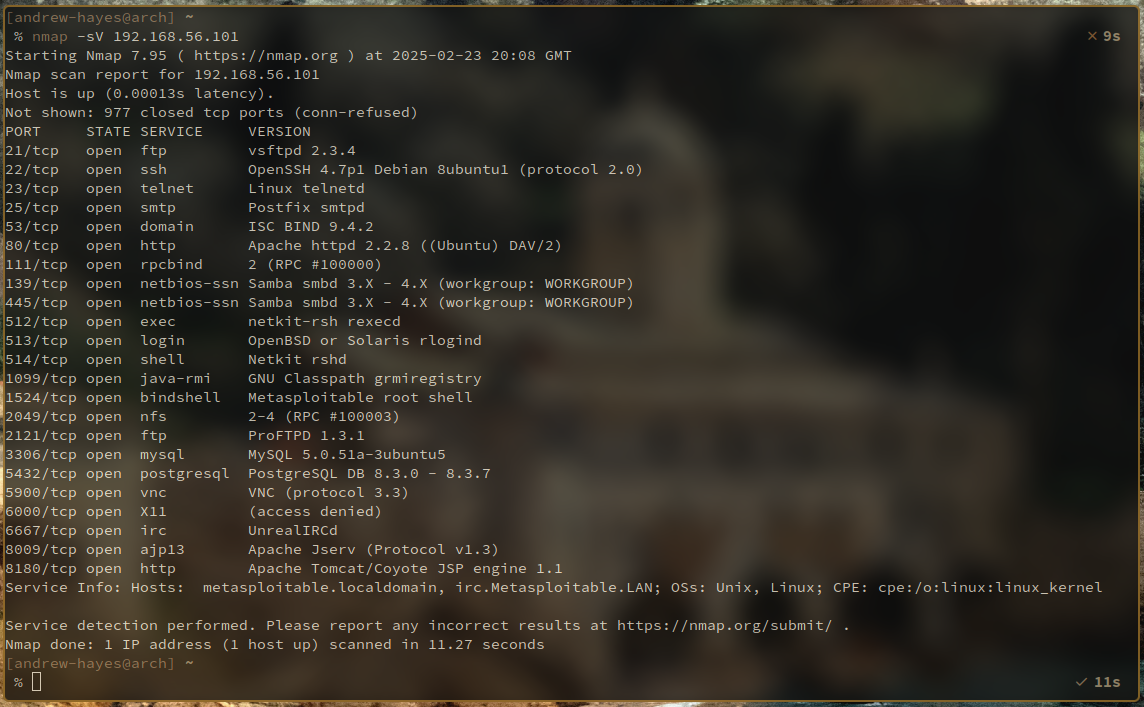
\includegraphics[width=0.8\textwidth]{./images/nmap.png}
    \caption{Output of \texttt{nmap}}
\end{figure}
\end{frame}

\begin{frame}{Exploit 1: FTP}
    Seeing that there was a FTP service running using \texttt{vsftpd 2.3.4}, I then searched for this service in the Metasploit console and saw that there was a backdoor exploit for this particular version of \texttt{vsftpd}:

\begin{figure}[H]
    \centering
    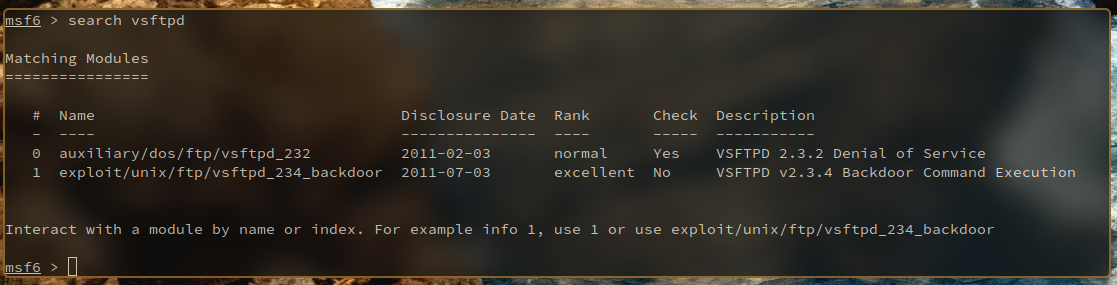
\includegraphics[width=\textwidth]{./images/searchftp.png}
    \caption{Output of \texttt{search vsftpd} in \texttt{msfconsole}}
\end{figure}
\end{frame}

\begin{frame}{Exploit 1: FTP}
    I then set the \texttt{RHOST} value and ran the exploit:

\begin{figure}[H]
    \centering
    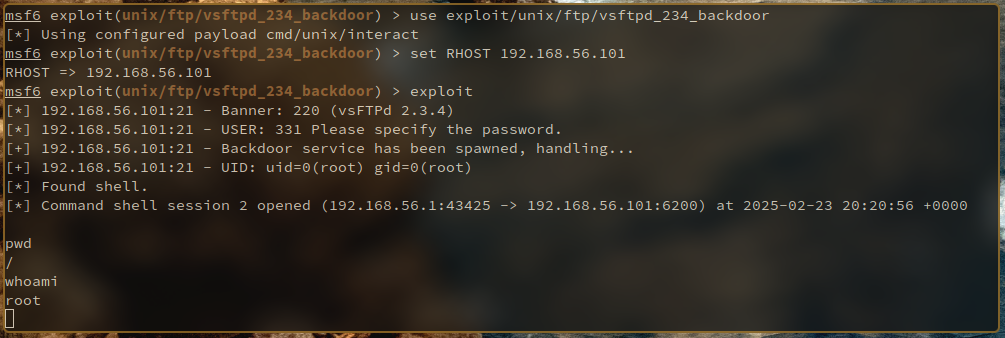
\includegraphics[width=\textwidth]{./images/ftpexploit.png}
    \caption{Results of running \texttt{use exploit/unix/ftp/vsftpd\_234\_backdoor}}
\end{figure}
\end{frame}

\begin{frame}{Exploit 1: FTP}
    \begin{itemize}
        \item   As can be seen from the output on the previous slide, this backdoor exploit gives us remote root access to the vulnerable Metasploitable2 machine -- a highly dangerous vulnerability.
        \item   This works because version \texttt{2.3.4} of the \texttt{vsftpd} program was shipped with a malicious backdoor inserted into the binary that is triggered when a user attempts to login with a username ending in \texttt{:)} and opens a command shell on TCP port \texttt{6200}.
        \item   The Metasploit exploit module attempts to login with a username ending in \texttt{:)}, triggering the backdoor, and then connects to port \texttt{6200}, thus giving the malicious user root access to the target system.
    \end{itemize}
\end{frame}

\begin{frame}{Exploit 2: Samba}
    Seeing from the \texttt{nmap} output that there is a Samba service running, I then searched for this service in the Metasploit console and saw that there were more than 70 possible exploits using Samba.
    One in particular caught my eye, that being the \texttt{exploit/multi/samba/usermap\_script} module, as it had rank ``Excellent'' and allows the attacker to gain shell access to the target system.
\end{frame}

\begin{frame}{Exploit 2: Samba}
    If you run \texttt{use exploit/multi/samba/usermap\_script} and then \texttt{show payloads} to see what payloads are available, 
    you will get a list of 44 payloads.

\begin{figure}[H]
    \centering
    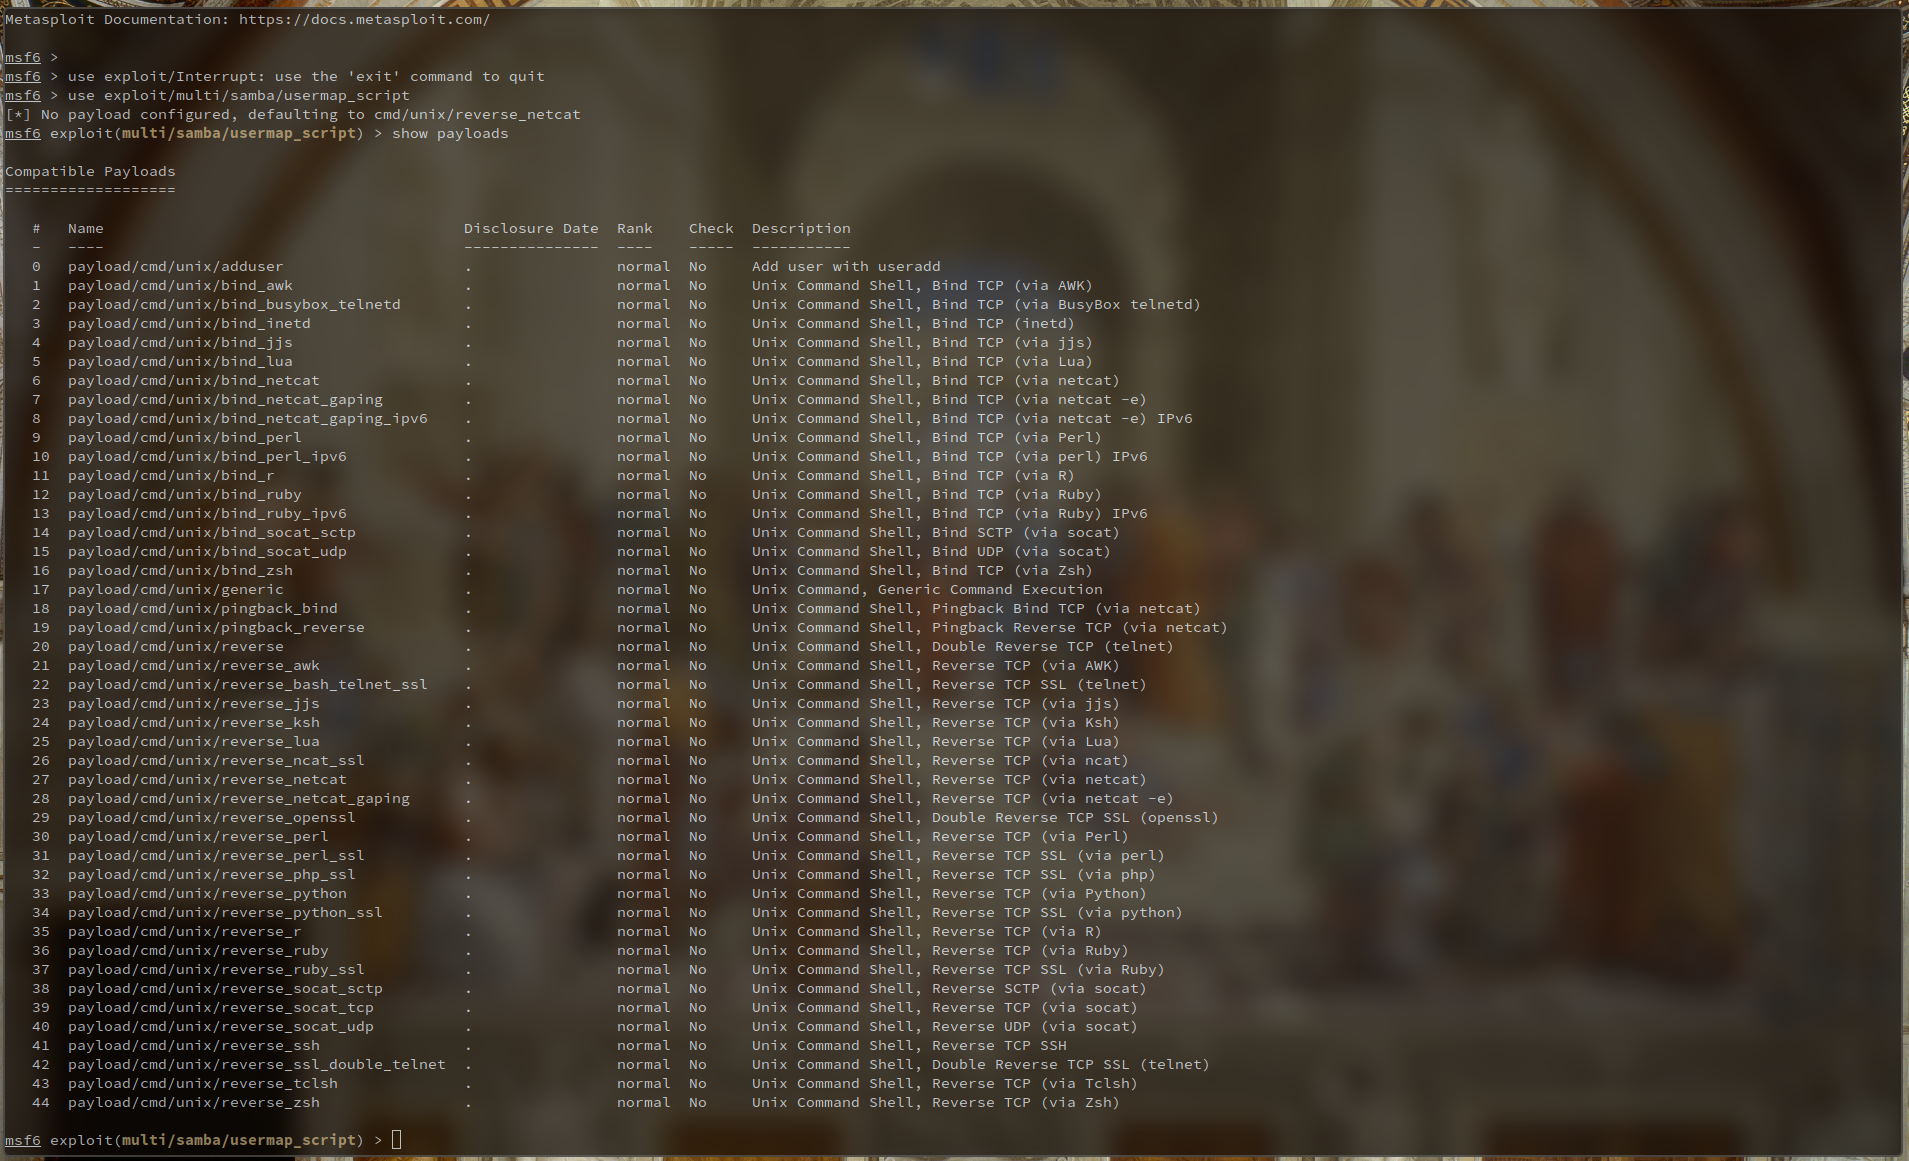
\includegraphics[width=0.8\textwidth]{./images/sambapayloads.png}
    \caption{Available payloads}
\end{figure}

\end{frame}

\begin{frame}{Exploit 2: Samba}
I chose the payload \texttt{payload/cmd/unix/bind\_netcat}, which spawns a shell on the target machine and binds it to a port with \texttt{netcat}, allowing the attacker to connect.
I then set the \texttt{RHOST} and ran the exploit.

\begin{figure}[H]
    \centering
    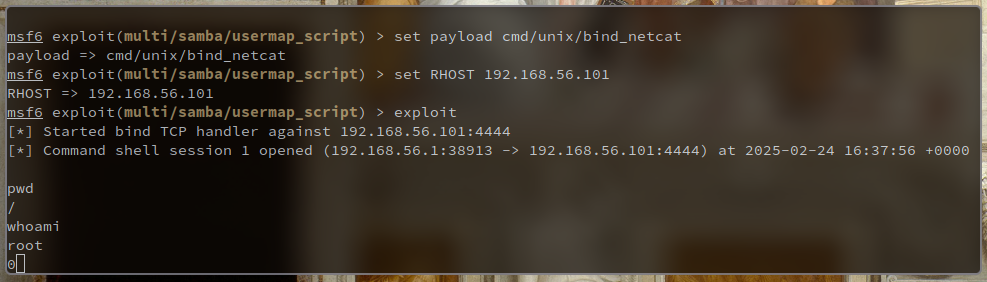
\includegraphics[width=\textwidth]{./images/sambaexploit.png}
    \caption{Running the exploit with \texttt{bind\_netcat} payload}
\end{figure}
\end{frame}

\begin{frame}{Exploit 2: Samba}
    \begin{itemize}
        \item   As can be seen from the output on the previous slide, this backdoor also gives us remote root access to the target machine.
        \item   This exploit works because Samba allows administrators to map incoming usernames to different local users using the \texttt{username map} feature, which processes the incoming usernames using a shell command.
        \item   In certain vulnerable versions of Samba, the user input is not sanitised properly and an attacker can insert special characters to inject arbitrary shell commands, such as spawning a \texttt{netcat} shell on a specific port.
    \end{itemize}
\end{frame}

\begin{frame}{Exploit 3: \texttt{distcc}}
The final exploit that I tested was one that exploited a command injection vulnerability in the program \texttt{distcc}, a program which allows the distributed compilation of C/C++ programs.

\begin{figure}[H]
    \centering
    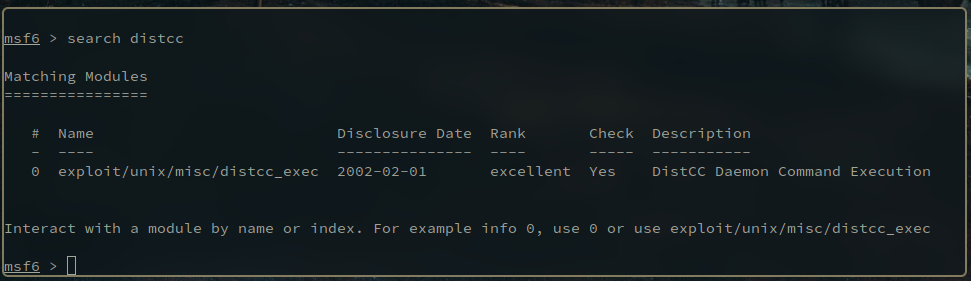
\includegraphics[width=\textwidth]{./images/distccsearch.png}
    \caption{Output of \texttt{search distcc}}
\end{figure}
\end{frame}

\begin{frame}{Exploit 3: \texttt{distcc}}
There are 14 payloads to choose from with this exploit, both that bind shells and that create reverse shells.
I chose the \texttt{cmd/unix/bind\_perl} payload, as it binds a shell allowing arbitrary execution of commands.

\begin{figure}[H]
    \centering
    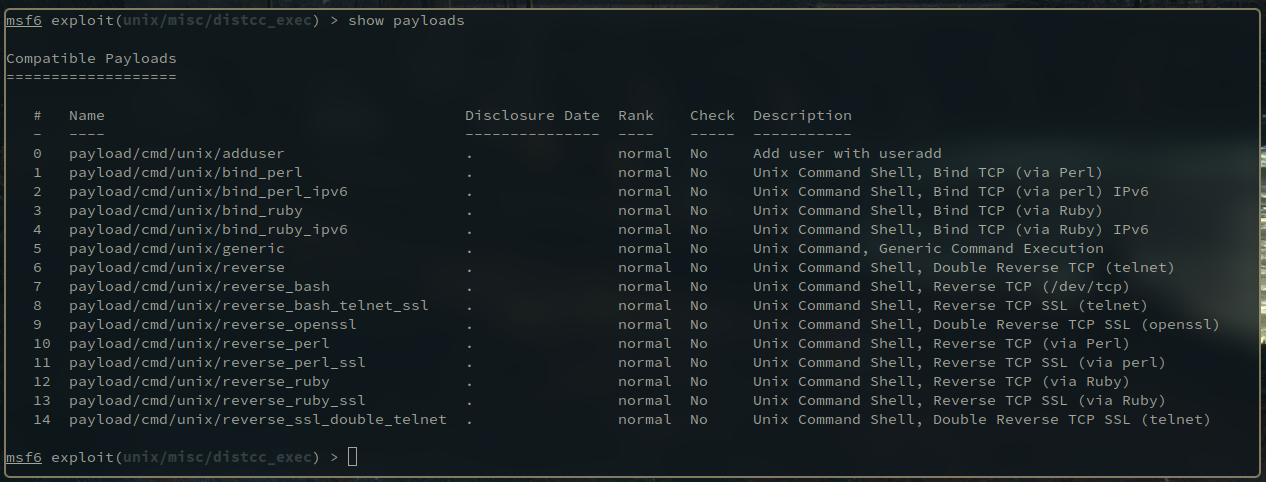
\includegraphics[width=\textwidth]{./images/distccpayloads.png}
    \caption{Output of \texttt{show payloads}}
\end{figure}
\end{frame}

\begin{frame}{Exploit 3: \texttt{distcc}}
Once I had selected my payload, I set the \texttt{RHOST} variable and ran the exploit:

\begin{figure}[H]
    \centering
    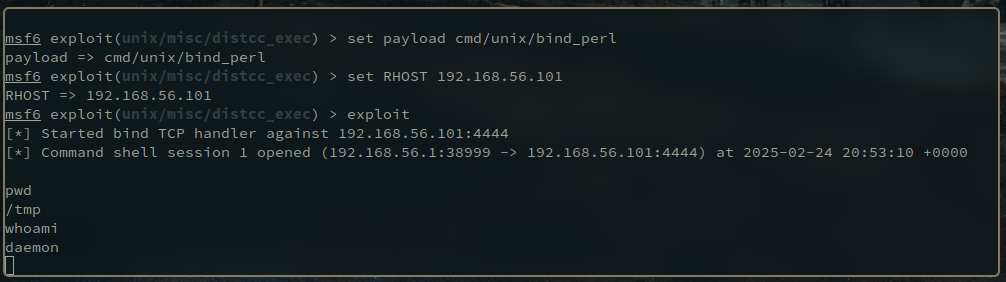
\includegraphics[width=\textwidth]{./images/distccexploit.png}
    \caption{Running the exploit with the \texttt{bind\_perl} exploit}
\end{figure}
\end{frame}

\begin{frame}{Exploit 3: \texttt{distcc}}
\begin{itemize}
    \item   As can be seen from the output on the previous slide, this vulnerability establishes a connection to shell running on the target machine from which arbitrary commands can be executed.
    \item   However, as can also be seen from the previous slide, the output of the \texttt{whoami} command is not \texttt{root}, but rather \texttt{daemon};
            this user has fewer privileges than \texttt{root} and therefore is not as serious as the other two exploits.
    \item   Nonetheless, the vulnerability is still rather serious, and is possible on any version of \texttt{distcc} if input is not sanitised properly.
\end{itemize}
\end{frame}

\end{document}
